\section{Anhang - Jupyter Notebooks} \label{sec:anhang}

Da der Anhang eine gewisse Länge besitzt und in mehrere Abschnitte unterteilt werden kann, dient diese Seite als eine Art Inhaltsverzeichnis für ausschließlich den Anhang. Zu finden sind im Folgenden sämtliche Jupyter Notebooks zu den im Fließtext beschriebenen Funktionen und Fähigkeiten des Jetbot Roboterfahrzeugs.\\

\textbf{Grundlegende Funktionen:}\\
\hyperlink{page.27}{\textcolor{blue}{Steuern des Jetbot}}\\

\textbf{Kollisionsvermeidung:}\\
\hyperlink{page.32}{\textcolor{blue}{Datensammlung}}\\
\hyperlink{page.36}{\textcolor{blue}{Trainieren des CNN}}\\
\hyperlink{page.39}{\textcolor{blue}{Einsatz des trainierten Modells}}\\

\textbf{Spurverfolgung:}\\
\hyperlink{page.43}{\textcolor{blue}{Datensammlung}}\\
\hyperlink{page.47}{\textcolor{blue}{Trainieren des CNN}}\\
\hyperlink{page.51}{\textcolor{blue}{Einsatz des trainierten Modells}}\\

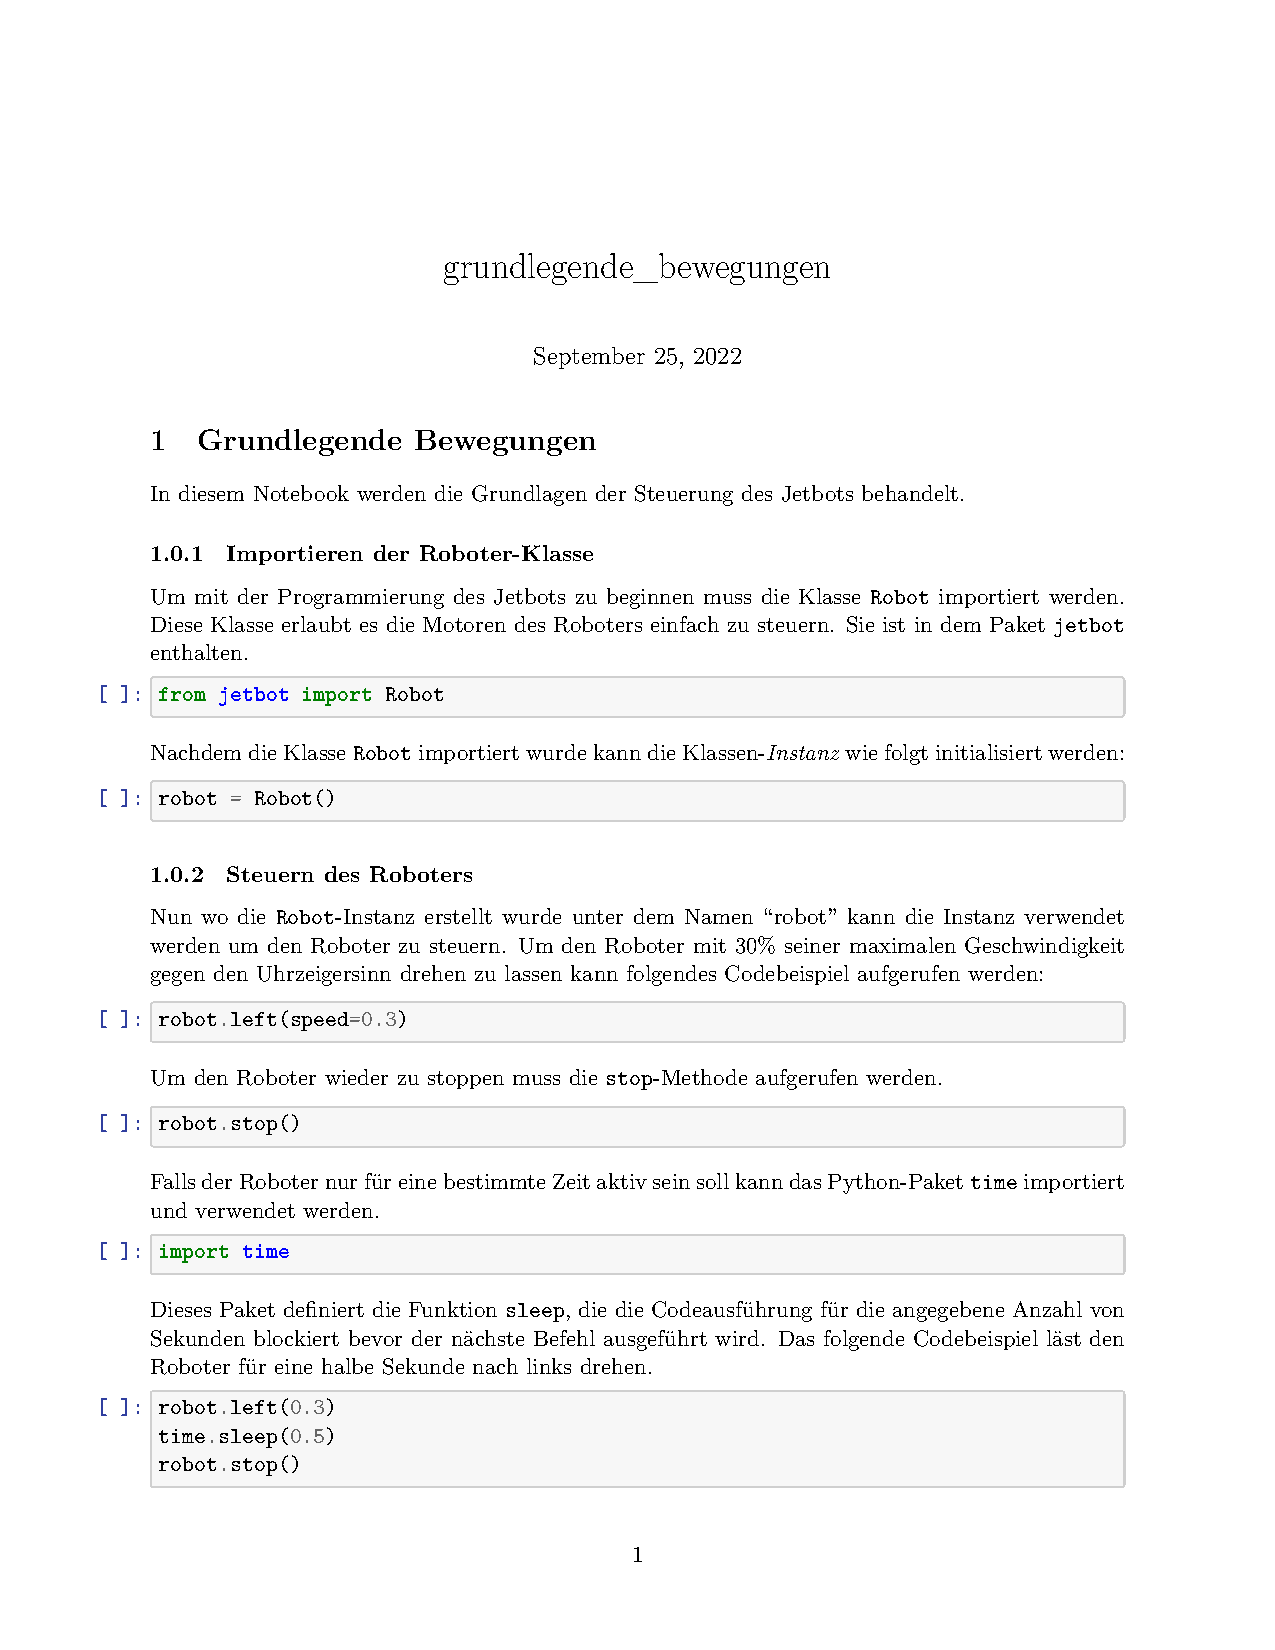
\includepdf[pages=-,angle=0]{Notebooks/grundlegende_bewegungen.pdf}


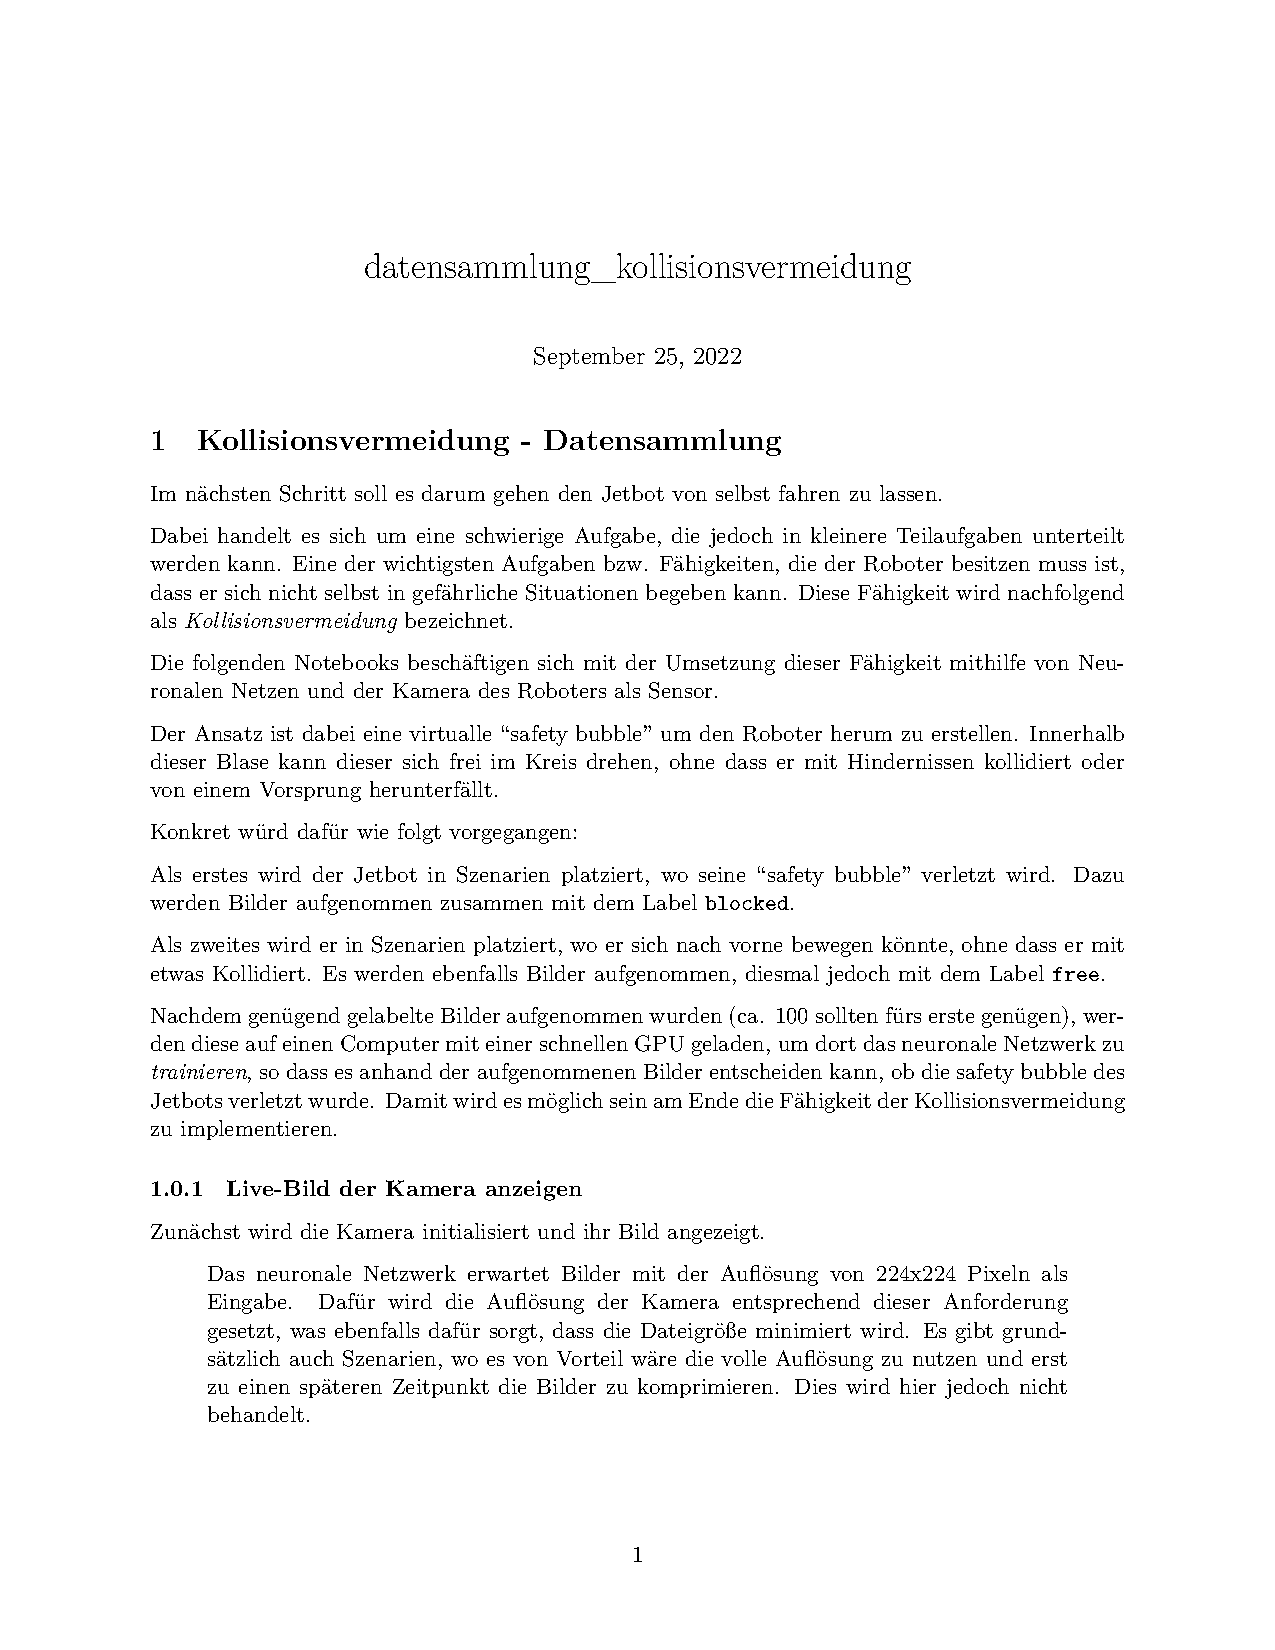
\includepdf[pages=-,angle=0]{Notebooks/datensammlung_kollisionsvermeidung.pdf}

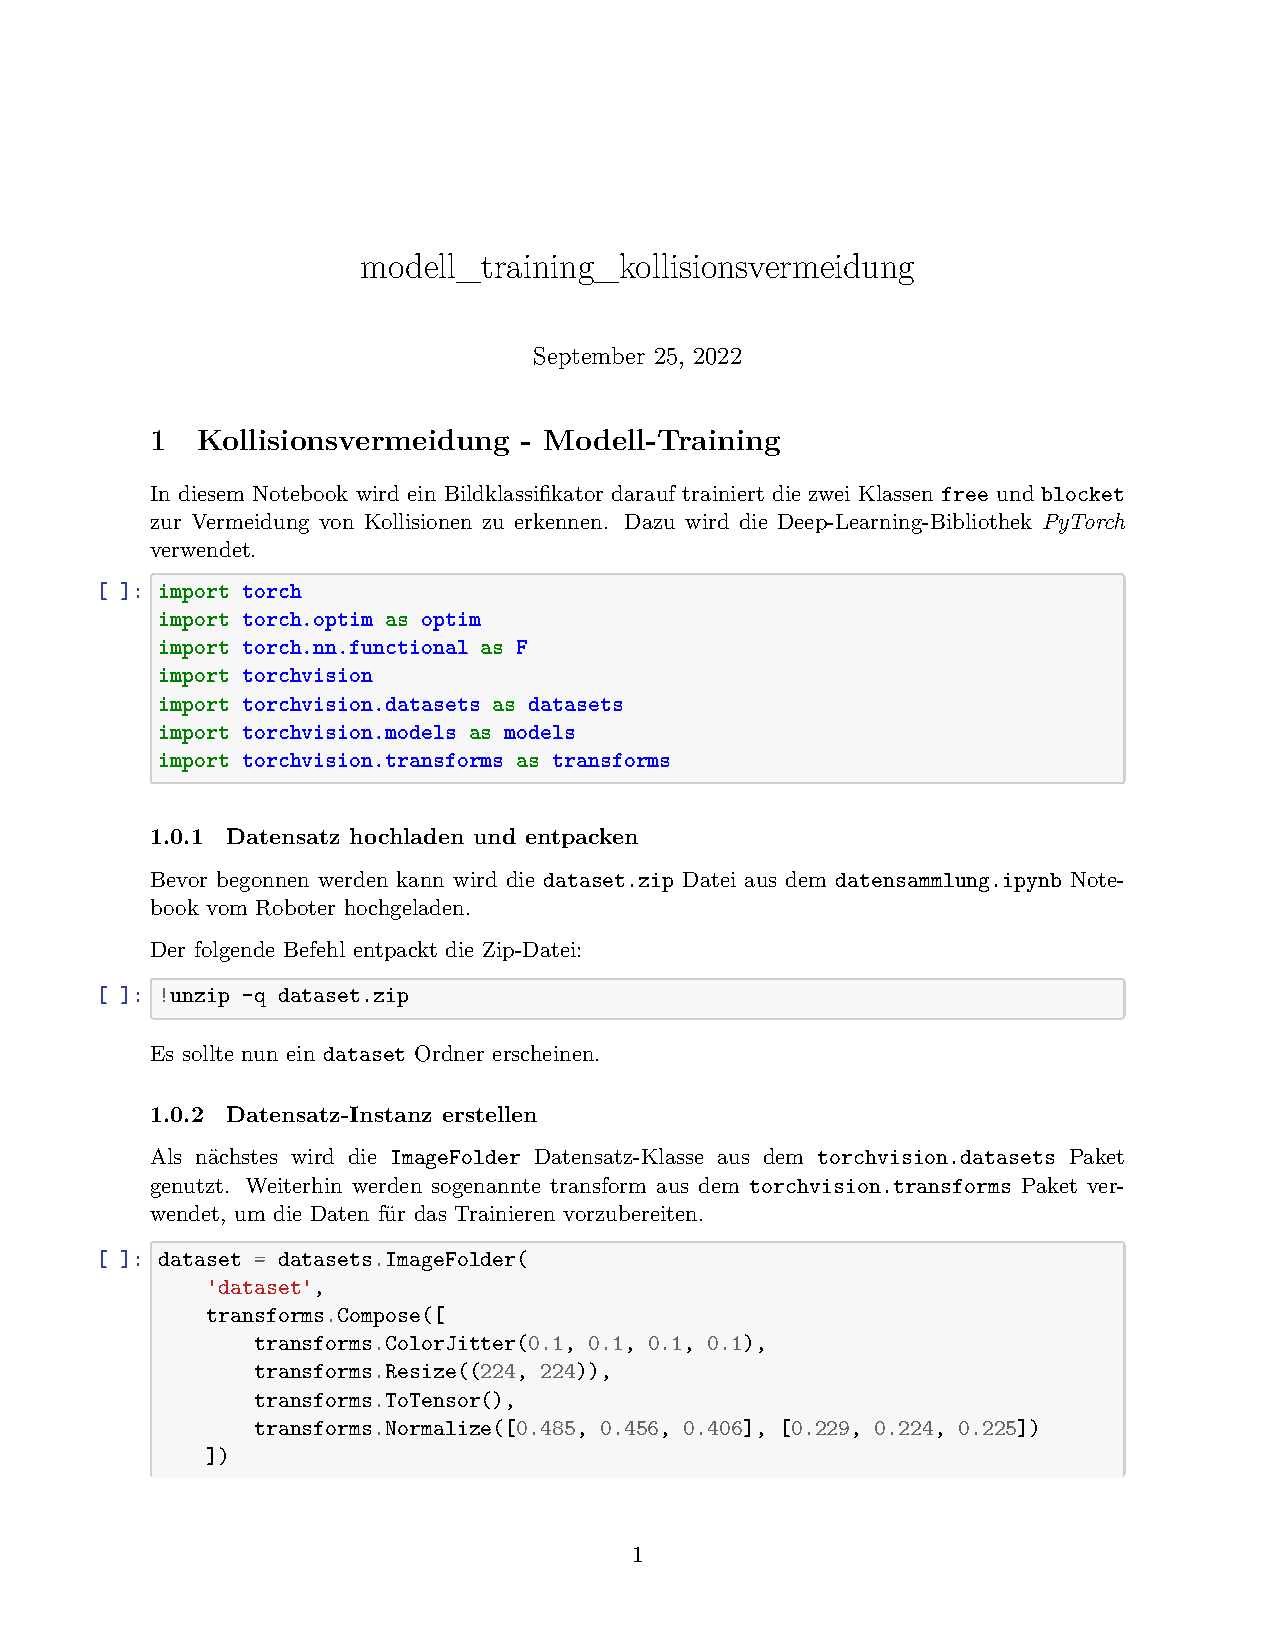
\includepdf[pages=-,angle=0]{Notebooks/modell_training_kollisionsvermeidung.pdf}

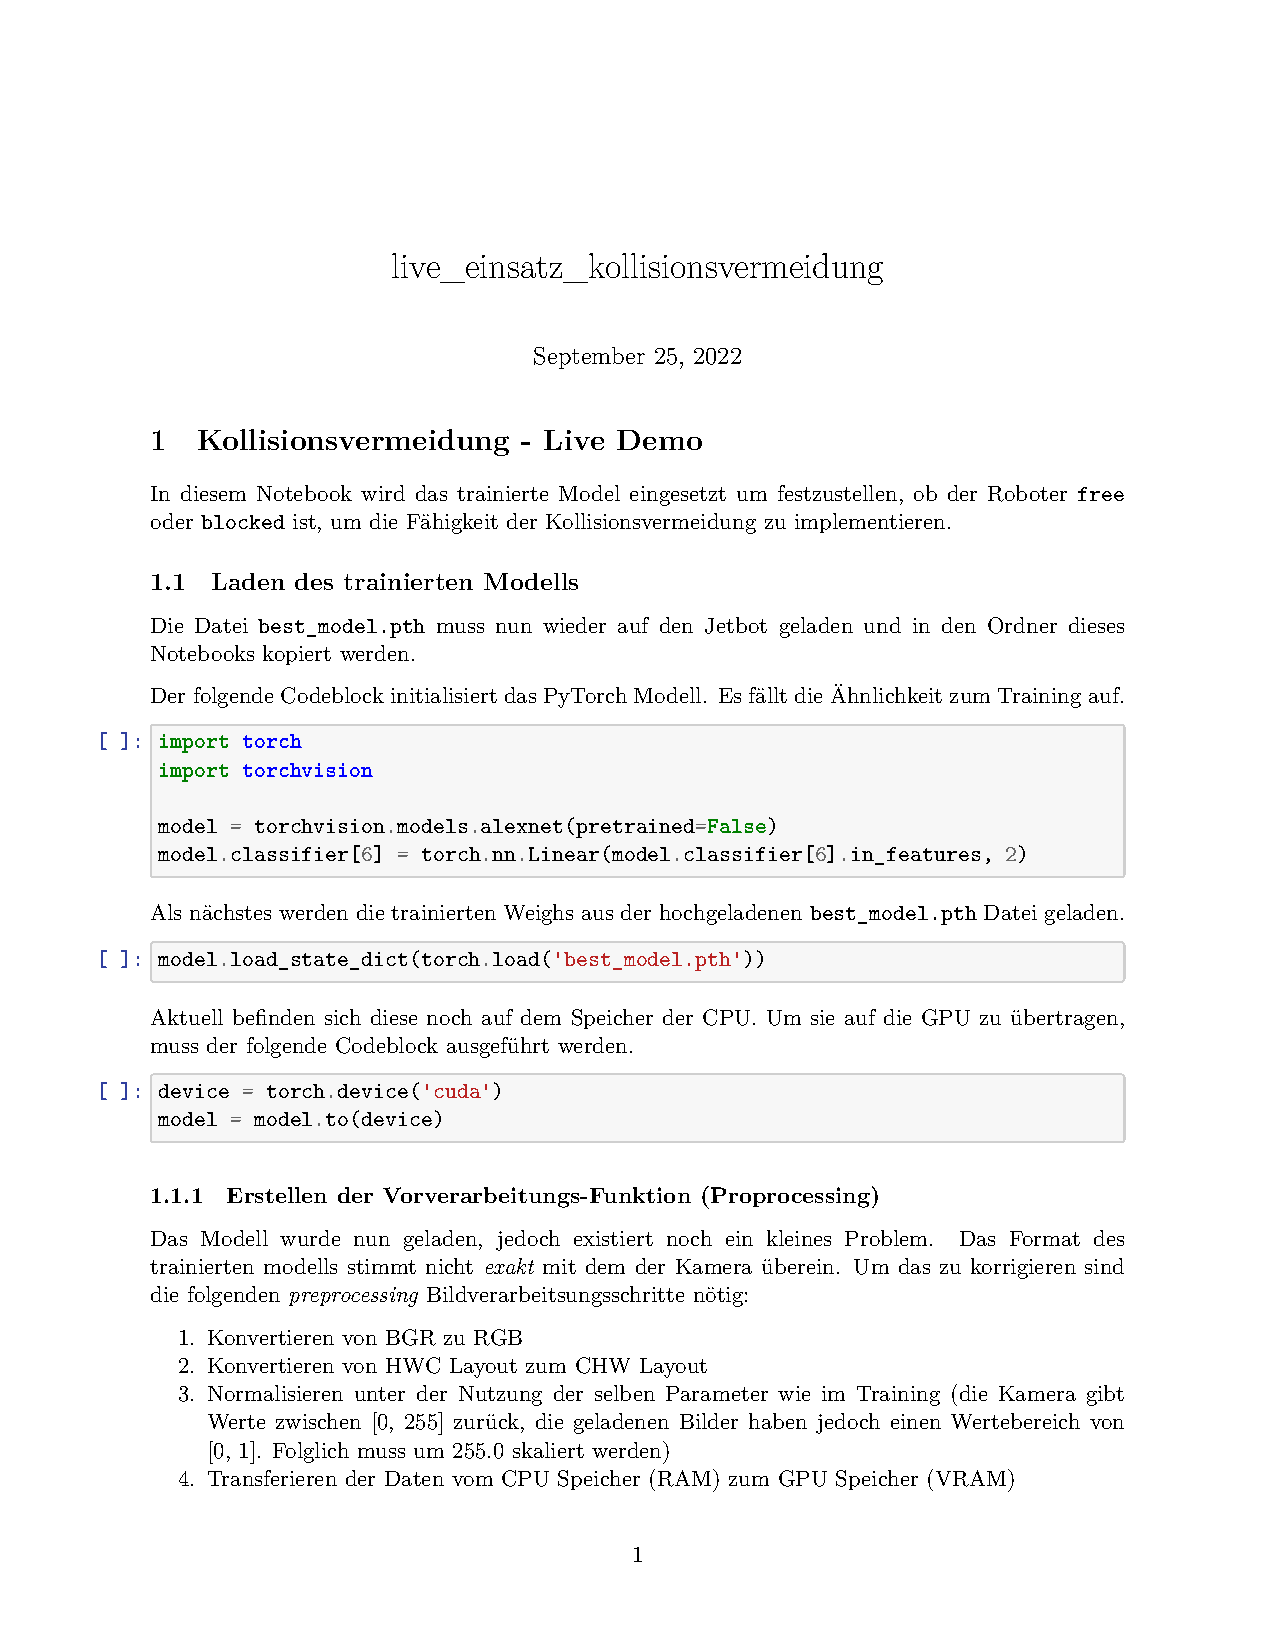
\includepdf[pages=-,angle=0]{Notebooks/live_einsatz_kollisionsvermeidung.pdf}


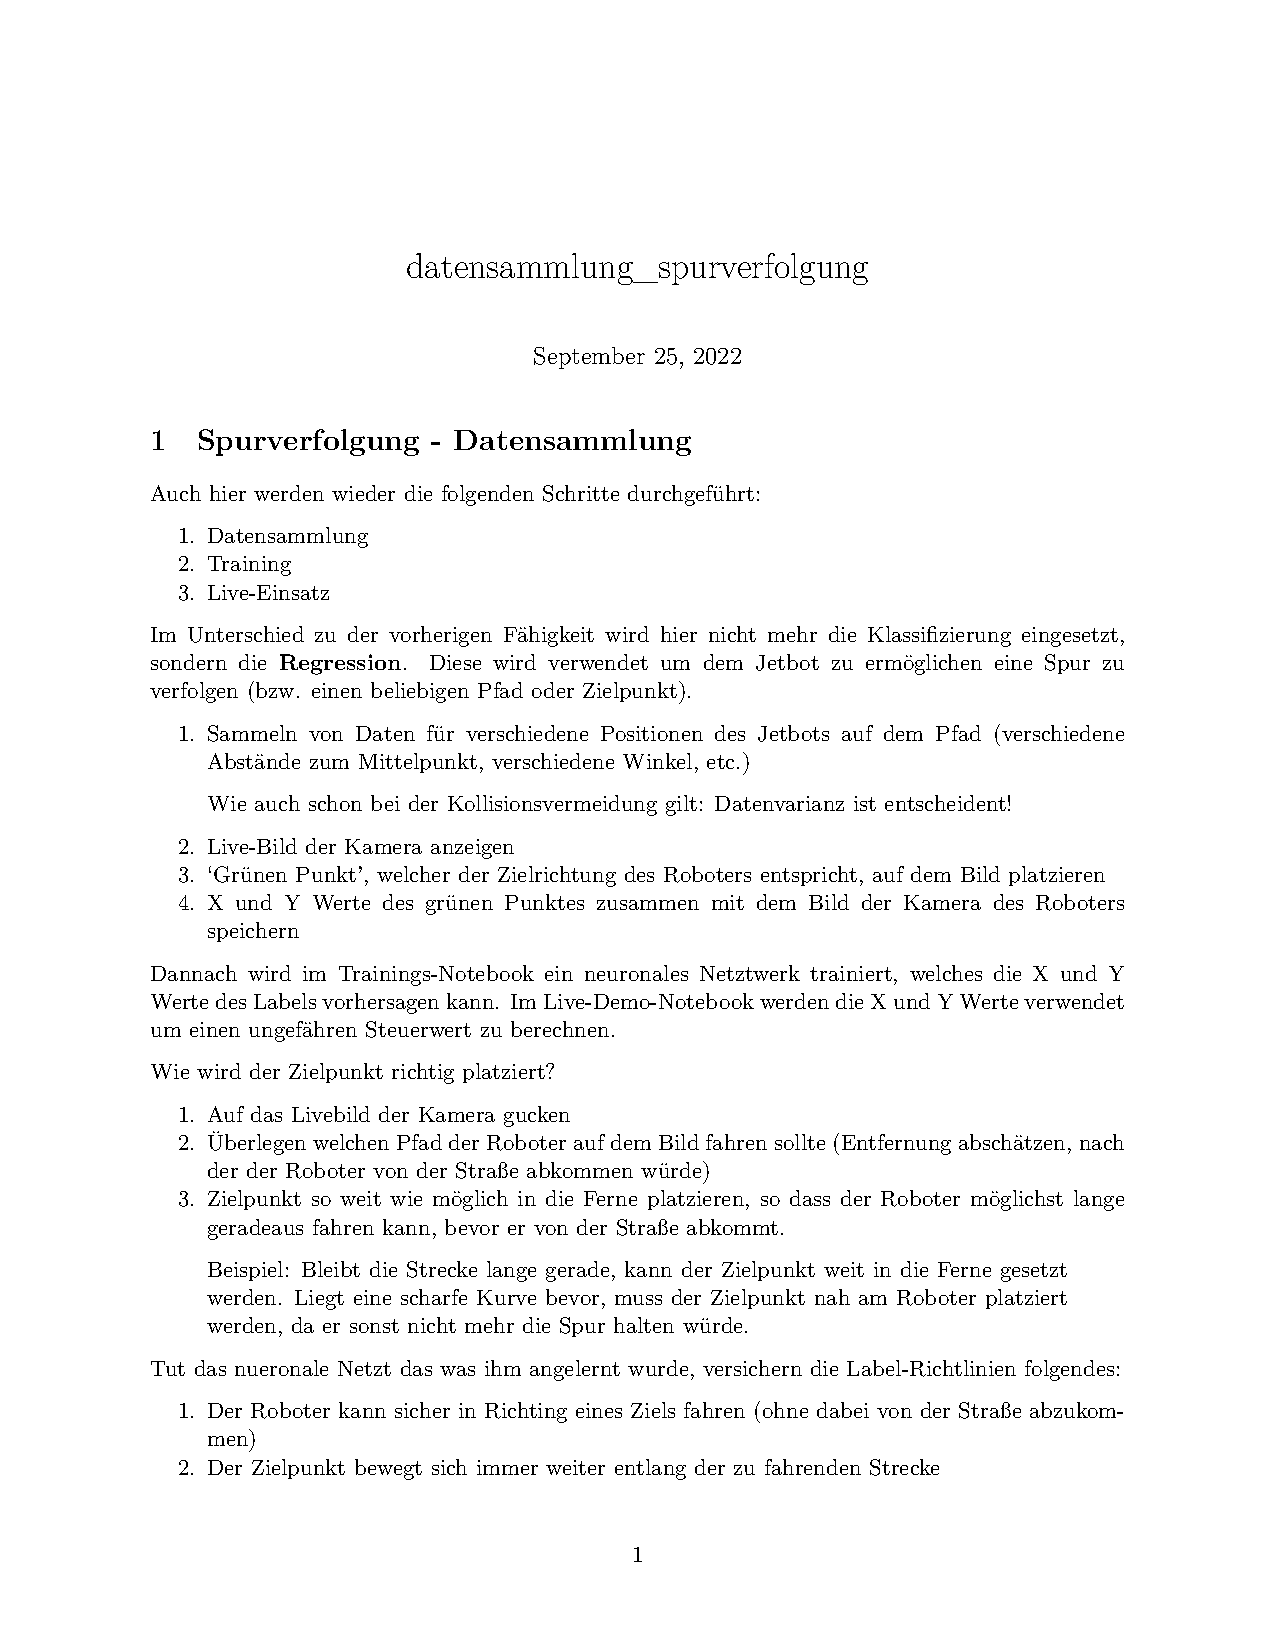
\includepdf[pages=-,angle=0]{Notebooks/datensammlung_spurverfolgung.pdf}

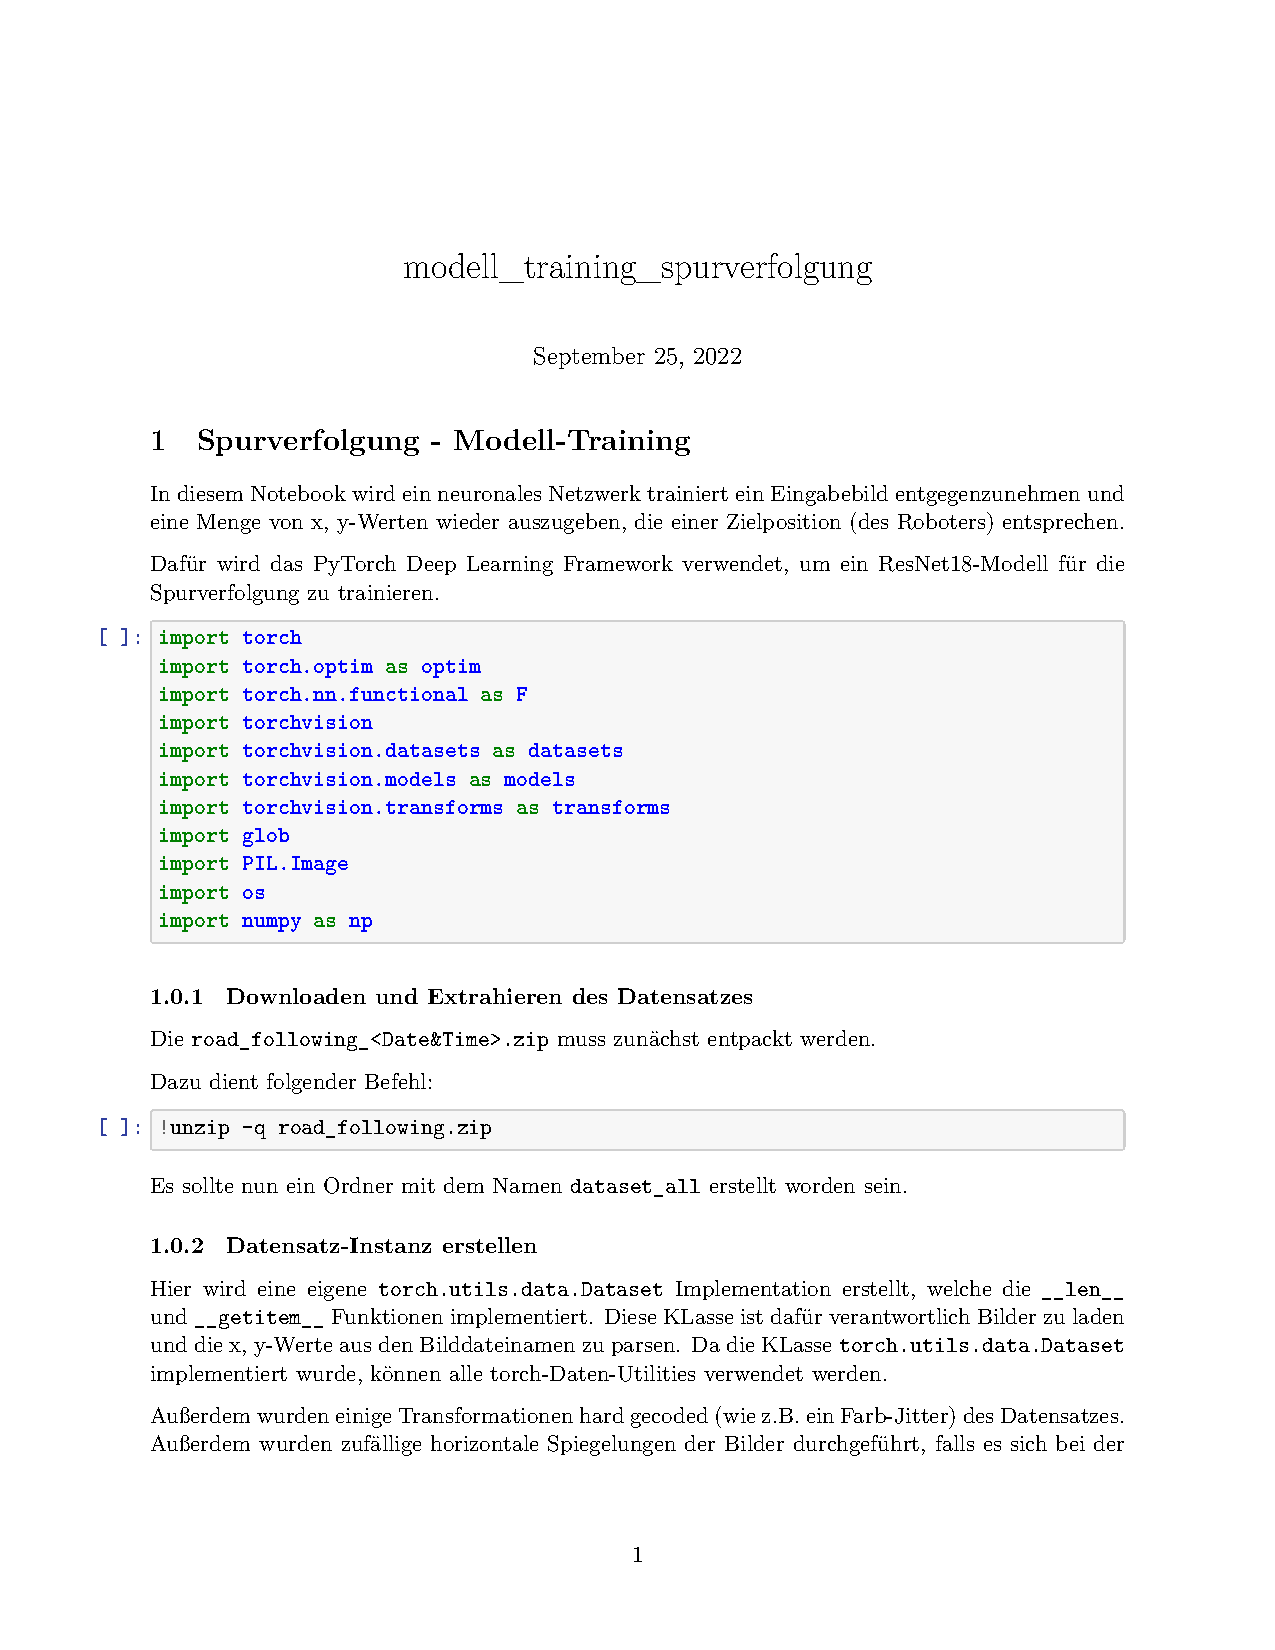
\includepdf[pages=-,angle=0]{Notebooks/modell_training_spurverfolgung.pdf}

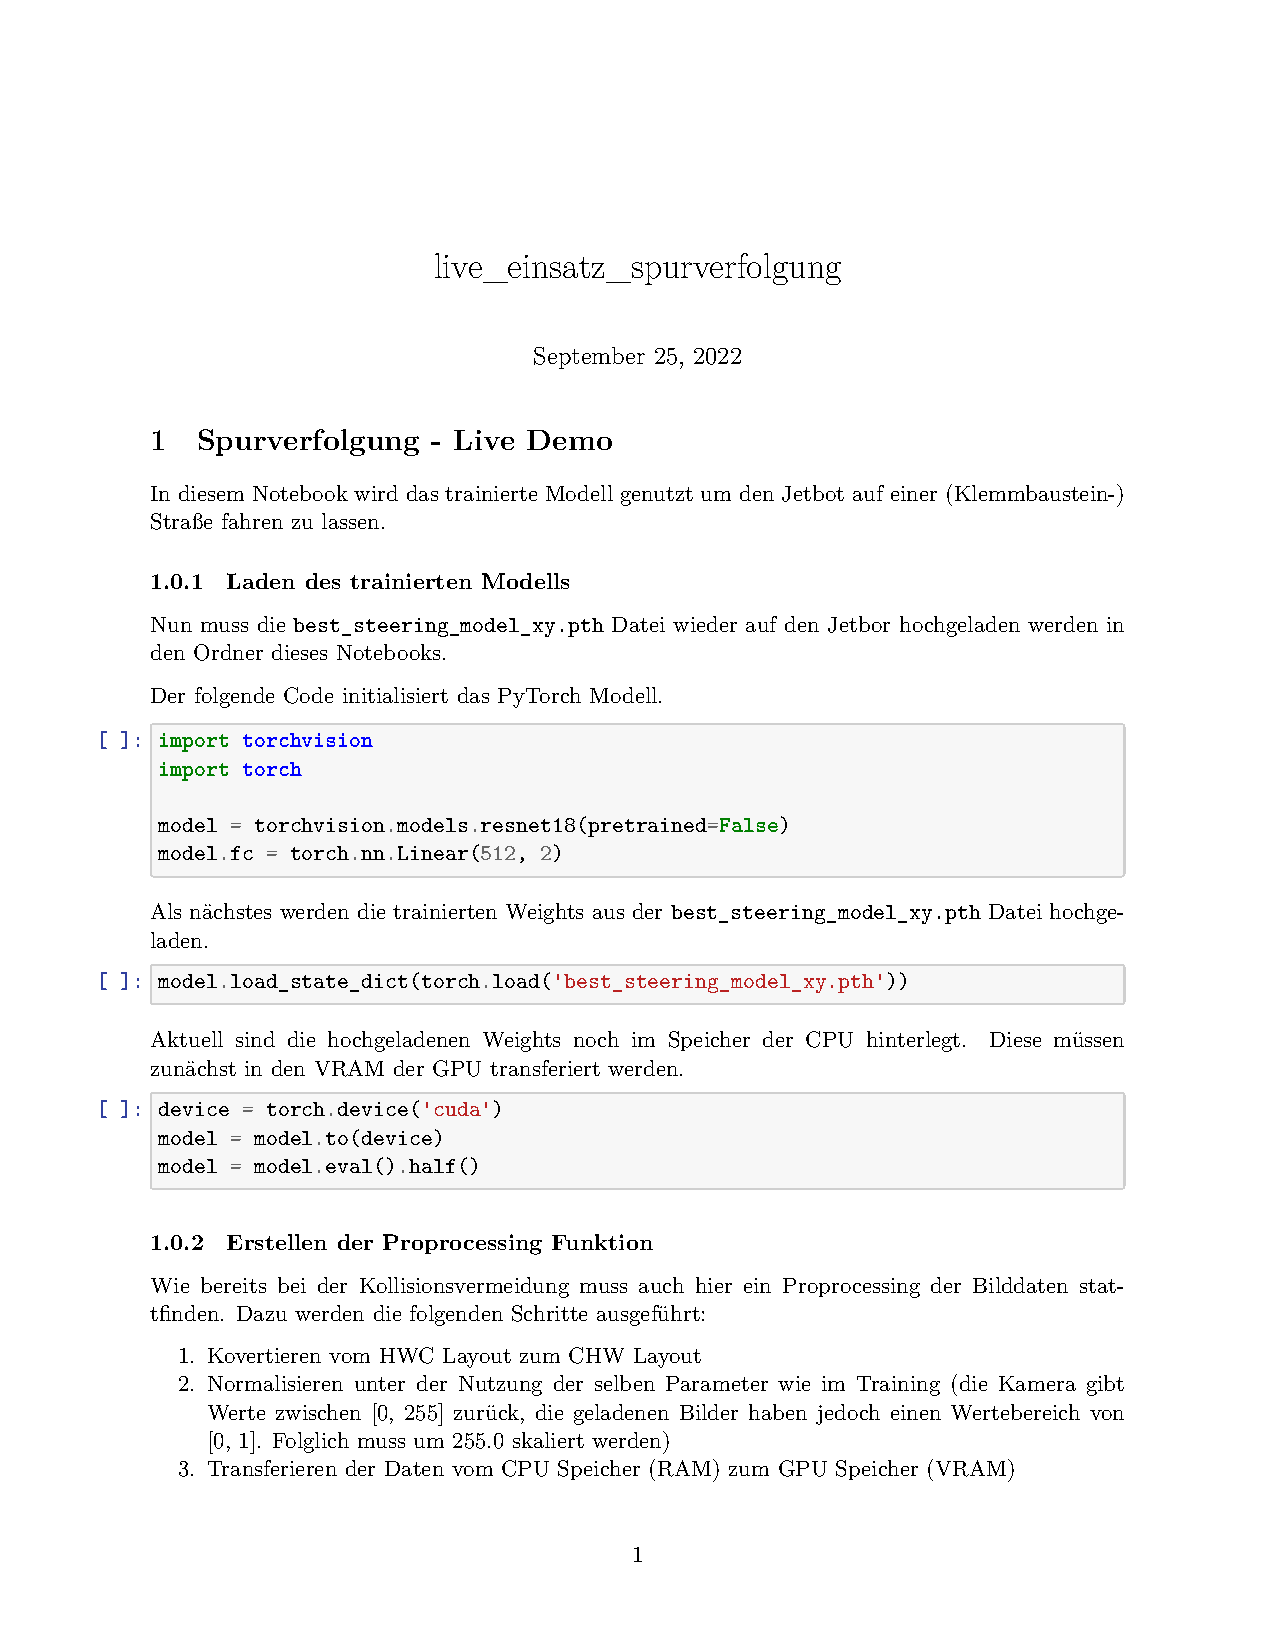
\includepdf[pages=-,angle=0]{Notebooks/live_einsatz_spurverfolgung.pdf}